\documentclass[12pt,compress,ngerman,utf8,t]{beamer}
\usepackage[ngerman]{babel}
\usepackage{calc}
\usepackage{ragged2e,wasysym,multicol,mathtools}
\usepackage[protrusion=true,expansion=true]{microtype}
\usepackage{booktabs}
\usepackage{multimedia}
\hypersetup{colorlinks=true}

\newcommand{\video}[2]{\movie[width=#2,height=#2,autostart,loop,poster]{}{#1}}

\graphicspath{{images/}}

\title[Fourdimensional geometry]{The curious world of \\ four-dimensional geometry}
\author[Ingo Blechschmidt, Matthias Hutzler]{\texorpdfstring{\scriptsize
\vspace*{-1em} \\
\textbf{Late Night Wondrous Mathematics at 35c3} \\
\emph{Questions are welcome at any point! Don't save them until the end.} \\
\medskip
\begin{minipage}{3cm}\centering Ingo Blechschmidt \\ Università di
Verona\end{minipage}\qquad
\begin{minipage}{3cm}\centering Matthias Hutzler \\ Universität Augsburg\end{minipage}}{Ingo Blechschmidt and Matthias
Hutzler}}


%\usetheme{Warsaw}
\useinnertheme[shadow=true]{rounded}
\useoutertheme{split}
\usecolortheme{orchid}
\usecolortheme{whale}
\setbeamerfont{block title}{size={}}

\useinnertheme{rectangles}

\usecolortheme{seahorse}
\definecolor{mypurple}{RGB}{150,0,255}
\setbeamercolor{structure}{fg=mypurple}
\definecolor{myred}{RGB}{150,0,0}
\setbeamercolor*{title}{bg=myred,fg=white}
\setbeamercolor*{titlelike}{bg=myred,fg=white}

\usefonttheme{serif}
\usepackage[T1]{fontenc}
\usepackage{libertine}

\setbeamertemplate{navigation symbols}{}

\setbeamertemplate{title page}[default][colsep=-1bp,rounded=false,shadow=false]
\setbeamertemplate{frametitle}[default][colsep=-2bp,rounded=false,shadow=false,center]

\newcommand{\hil}[1]{{\usebeamercolor[fg]{item}{\textbf{#1}}}}
\setbeamertemplate{frametitle}{%
  \vskip1em%
  \leavevmode%
  \begin{beamercolorbox}[dp=1ex,center]{}%
      \usebeamercolor[fg]{item}{\textbf{\textsf{\Large \insertframetitle}}}
  \end{beamercolorbox}%
}

\setbeamertemplate{footline}{%
  \leavevmode%
  \hfill%
  \begin{beamercolorbox}[ht=2.25ex,dp=1ex,right]{}%
    \usebeamerfont{date in head/foot}
    \insertframenumber\,/\,\inserttotalframenumber\hspace*{1ex}
  \end{beamercolorbox}%
  \vskip0pt%
}

\setbeameroption{hide notes}
\setbeamertemplate{note page}[plain]

\begin{document}

\begin{frame}
  \centering
  \includegraphics[width=0.4\textwidth]{great-grand-120-cell}
  \smallskip

  \titlepage
\end{frame}


\section{Basics}

\begin{frame}[plain,c]
  \centering
  \Large
  \hil{How does the sequence continue?}

  1, \pause $\infty$, \pause 5, \pause 6, \pause \hil{??}
\end{frame}
\addtocounter{framenumber}{-1}


\subsection{Four dimensions: what?}

\begin{frame}{Four dimensions?}
  \centering
  \only<1>{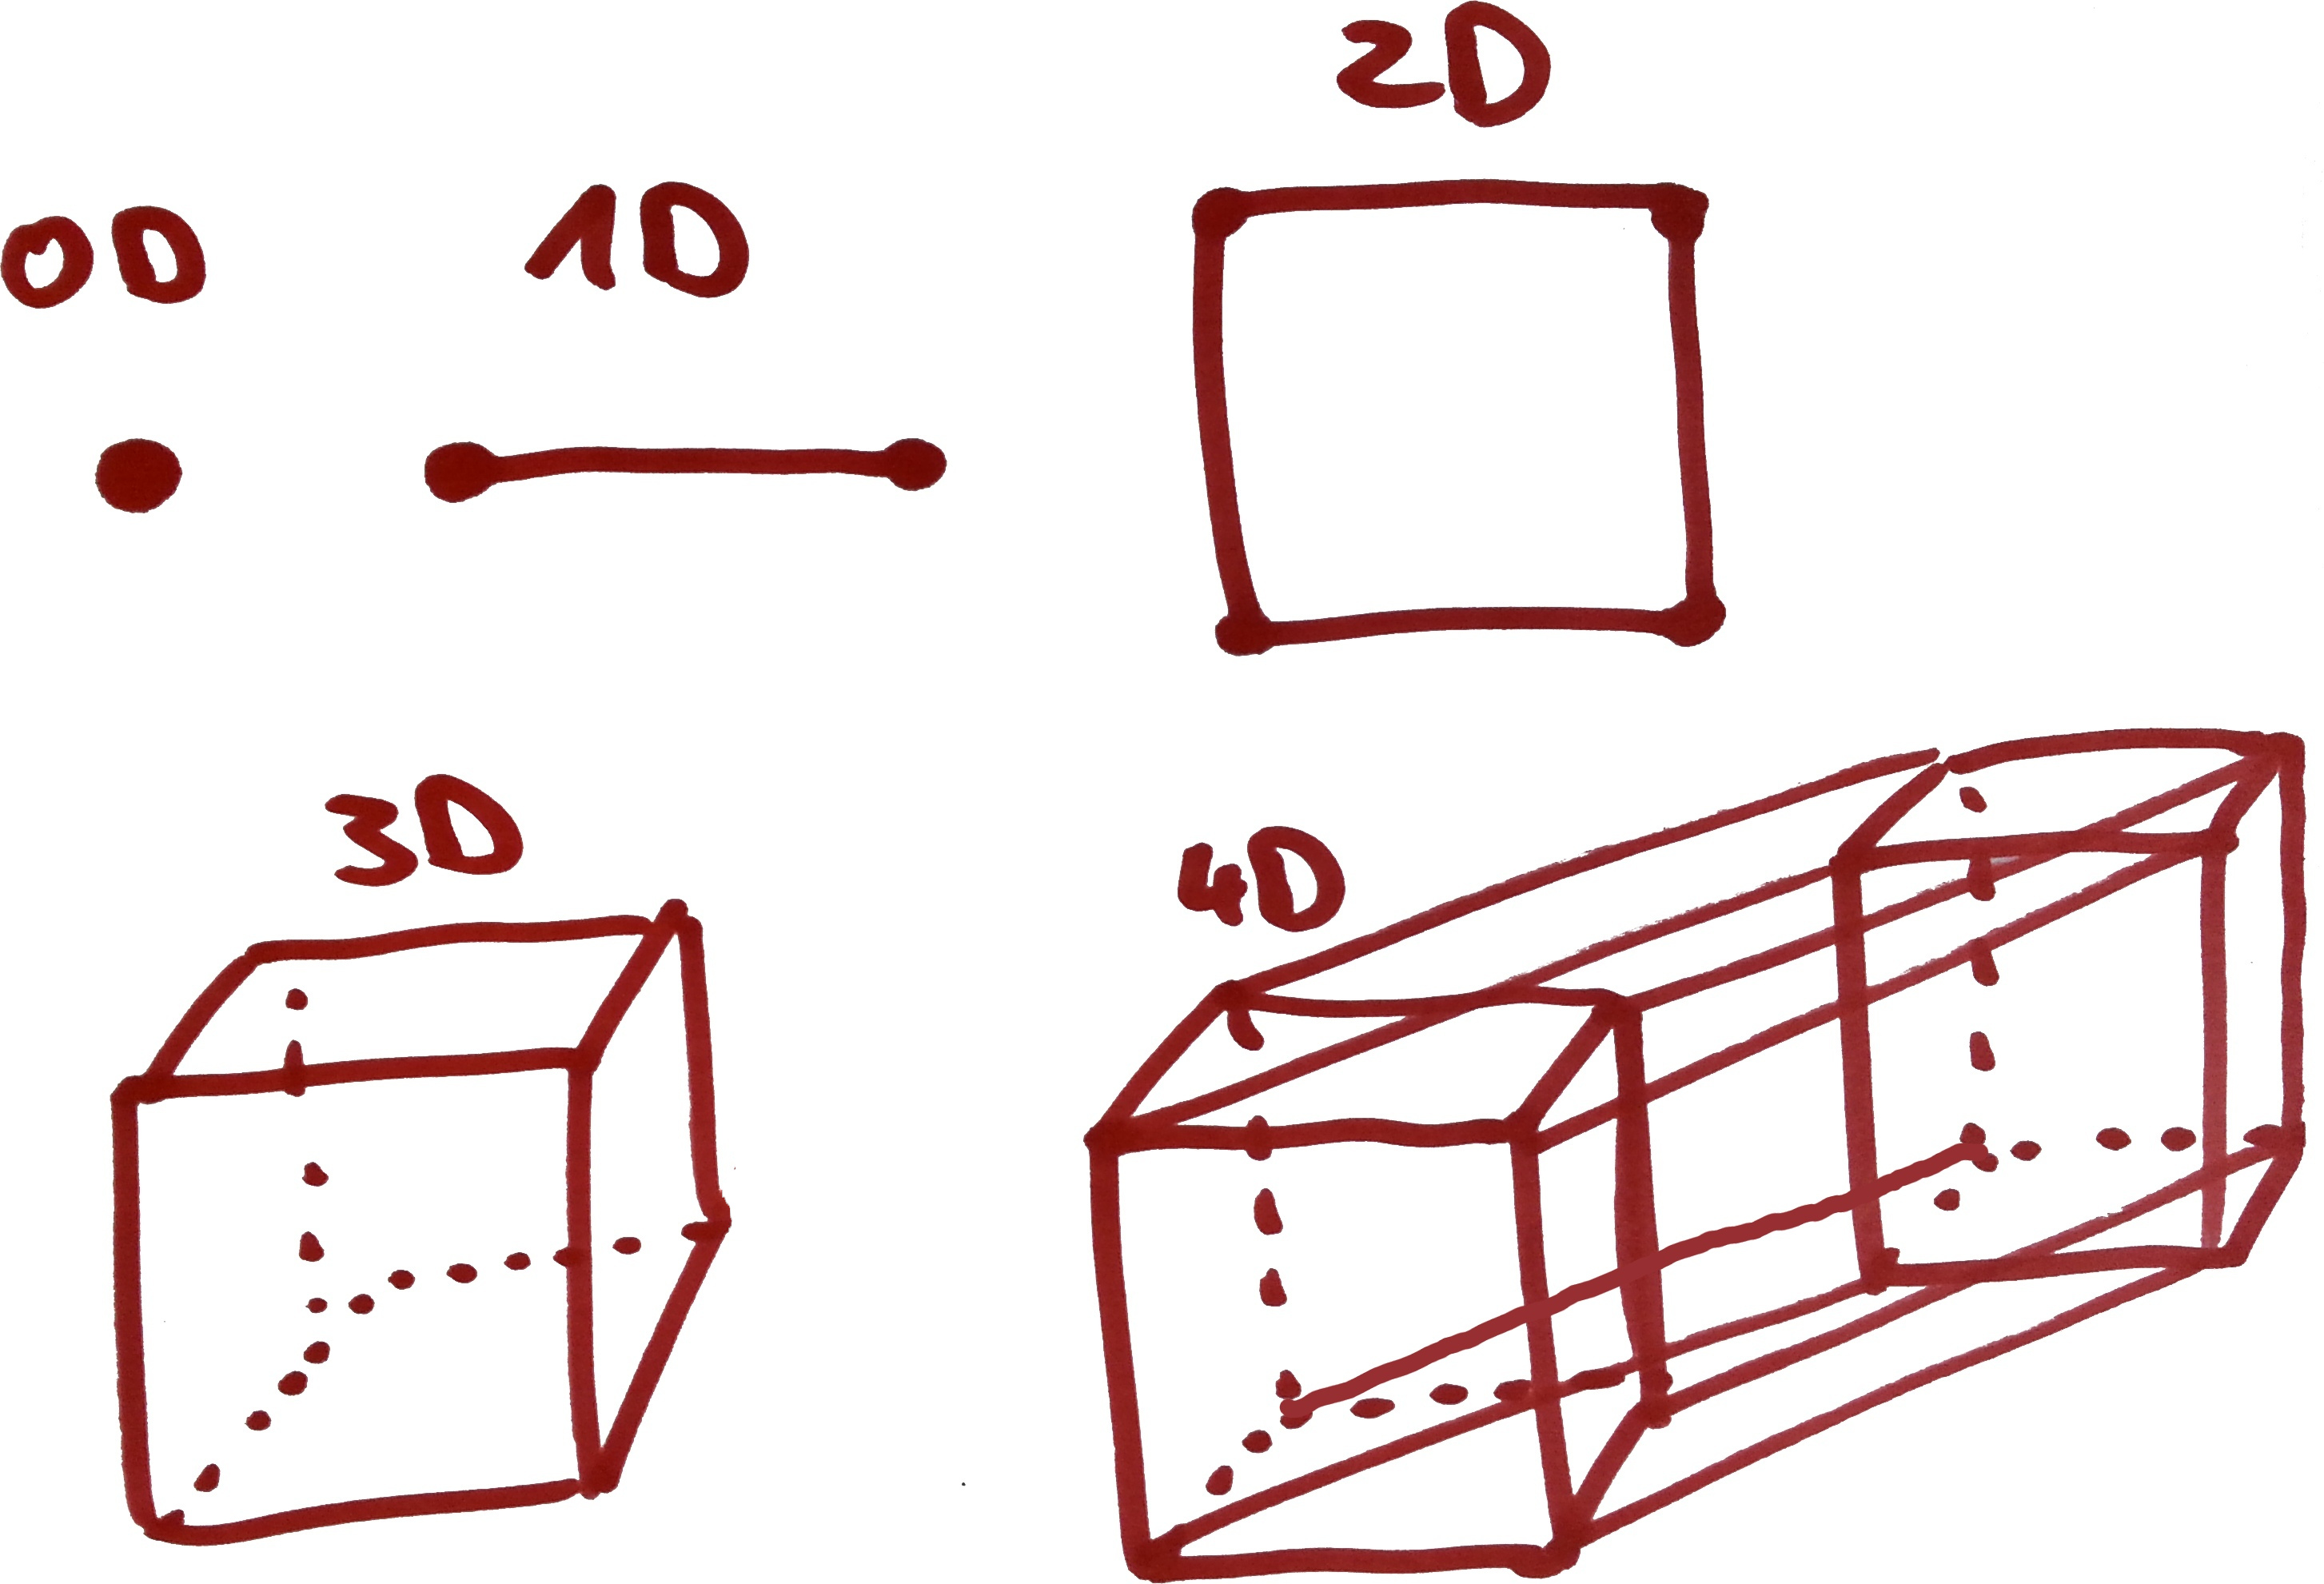
\includegraphics[width=0.9\textwidth]{4d-tesseract}}
  \only<2>{\includegraphics[width=0.9\textwidth]{4d-pentachoron}}
  \only<3>{\includegraphics[width=0.9\textwidth]{prisoner}}
  \par
  % Skizze Punkt, Linie, Quadrat, Würfel, nach \pause Tesserakt
  % Skizze Punkt, Linie, Dreieck, Tetraeder, 4-dimensionales Simplex
  % Sache mit Projektion erklären
  % klarstellen, dass wir über vierdimensionalen Raum (nicht Raum+Zeit) sprechen
  % nicht: 11-dimensionaler Quantenschaum
  % Wo erkennt man die drei Dimensionen in der realen Welt?
  % Gefängnisse (Quadrat genügt im Flachland, Würfel genügt in 3D, genügt nicht in 4D)
\end{frame}

\note{
  \begin{itemize}
    \item On the previous slide you see two-dimensional projections of the
    three-dimensional cube and the four-dimensional hypercube (tesseract).
    \item We're talking about four spatial dimensions. This is not related to
    four-dimensional spacetime or eleven-dimensional string theory.
    \item A flatlander can be imprisoned by enclosing them with a square. But
    we, as three-dimensional beings, can free them by grabbing them, lifting
    them up in the third dimension, moving them a little to the side, and
    putting them back into flatland.
    \item Similarly, a four-dimensional being could free us if we were imprisoned
    in a three-dimensional cube.
  \end{itemize}
}


\subsection{Knot theory}

\begin{frame}{Tying your shoelaces}
  % Erklären, dass Schnürsenkel immer aufgehen würden
  \centering
  \includegraphics[width=0.65\textwidth]{trefoil-knot}
  \par
\end{frame}

\note{
  \begin{itemize}
    \item You can untie any knot in four dimensions. Two linked one-dimensional
    strings can always be separated in four dimensions.
    \item But it's possible to tangle an one-dimensional string with the
    two-dimensional surface of a sphere in four dimensions.
    \item More generally, in $n$ dimensions, one can tangle $a$-dimensional
    objects with $b$-dimensional objects provided that $a + b \geq n - 1$.
  \end{itemize}
}

%Verhedderbar
%in 3D: Schnur, Schnur; 2, 2; 1, 1
%in 3D: Punkt, Fläche;  0, 1; 0, 2
%in 2D: Schnur, Punkt;  1, 2; 1, 0
%in 4D: Schnur, Fläche; 3, 2; 1, 2
%
%Beh.: Dimensionen addiert muss >= n - 1 sein, damit Verhedderung möglich ist
%
%Nicht verhedderbar
%in 3D: Punkt, Schnur; 3, 2; 0, 1
%in 3D: Punkt, Punkt;  3, 3; 0, 0
%in 4D: Punkt, Fläche      ; 0, 2
%in 4D: Schnur, Schnur     ; 1, 1


\section[Sizes]{Sizes in four dimensions}

\subsection{Hypervolume of hyperballs}

\begin{frame}{Hypervolume of hyperballs}
  \centering
  \vspace*{-0.5em}
  \includegraphics[width=0.4\textwidth]{sizes-1}
  \bigskip
  % vorher gscheite Definition der Hyperkugel
  % Bild vom Kreis im Quadrat
  % Bild vom Zylinder im Würfel
  % Bild von der Kugel im Würfel

  \small
  \begin{tabular}{lll}
    \toprule
    dimension & hypervolume & \\\midrule
    $n = 2$ & $\pi / 4$ & $\approx 0{.}785 \,\mathrm{m}^2$ \\
    $n = 3$ & $\pi / 6$ & $\approx 0{.}524 \,\mathrm{m}^3$ \\
    $n = 4$ & $\pi^2 / 32$ & $\approx 0{.}308 \,\mathrm{m}^4$ \\
    $n = 5$ & $\pi^2 / 60$ & $\approx 0{.}164 \,\mathrm{m}^5$ \\
    $n = 6$ & $\pi^3 / 384$ & $\approx 0{.}081 \,\mathrm{m}^6$ \\
    $n = 7$ & $\pi^3 / 840$ & $\approx 0{.}037 \,\mathrm{m}^7$ \\
    $n \to \infty$ & $\to 0$ \\
    \bottomrule
  \end{tabular}\par
\end{frame}

\note{
  \begin{itemize}
    \item The portion of the $n$-dimensional unit hypercube which is occupied
    by the inscribed $n$-dimensional hyperball gets arbitrary small in
    sufficiently high dimensions.
    \item The volume of such a hyperball is the answer to the following
    question: What is the probability that we managed to hit the hyperball with
    an dart, provided that we managed to hit the enclosing hyperball?
    \item Wikipedia gives
    \href{https://en.wikipedia.org/wiki/Volume_of_an_n-ball}{derivations for
    these formulas}.
    \item You can use the \emph{power of negative thinking} to motivate that
    the formula for the n-dimensional volume of the n-dimensional hyperball
    does \emph{not} contain $\pi^n$ (but rather $\pi^{\lfloor n/2 \rfloor}$):
    Think about the zero- and one-dimensional case.

    A zero-dimensional ball is just a point. Its zero-dimensional volume
    is~$1$.

    An one-dimensional ball is just a line segment. Its one-dimensional volume
    is its length.
  \end{itemize}
}


\subsection{Kissing hyperspheres}

\begin{frame}[plain,c]
  \centering\Huge
  \scalebox{2.6}{\hil{Love is}} \\[0.6em]
  \scalebox{2.6}{\hil{important.}}

  \bigskip
  \bigskip

  \scalebox{2.6}{\hil{$\boldsymbol{\heartsuit}$}}
  \par
\end{frame}
\addtocounter{framenumber}{-1}

\begin{frame}{Kissing hyperspheres}
  % Bild vier Kreise an den Ecken des Zweiheitsquadrats und Kreis in der Mitte
  \centering
  \vspace*{-1em}
  \includegraphics[width=0.3\textwidth]{sizes-2}
  \bigskip

  {\small
  \begin{tabular}{lll}
    \toprule
    dimension & radius of the inner hypersphere & \\\midrule
    $n = 2$ & \pause $\sqrt{2} - 1$ \\
    \pause
    $n = 3$ & \pause $\sqrt{3} - 1$ \\
    \pause
    $n = 4$ & $\sqrt{4} - 1$ \\
    \pause
    $n$ & $\sqrt{n} - 1$ \\
    \bottomrule
  \end{tabular}\par}
  \bigskip

  \centering
  \hil{The distance to the corners gets bigger and bigger.}
  \par
\end{frame}

\note{
  \begin{itemize}
    \item In two dimensions, the distance of a point~$(x,y)$ to the origin is
    $\sqrt{x^2 + y^2}$ (by the Pythagorean theorem).
    \item In three dimensions, the distance of a point~$(x,y,z)$ to the origin
    is~$\sqrt{x^2+y^2+z^2}$.
    \item The pattern continues to arbitrary dimensions.
    \item In four dimensions, the ``small hypersphere in the middle'' has
    exactly the same size as the hyperspheres at the 16 vertices of the
    hypercube.
    \item In even greater dimensions, the hyperspheres at the vertices are so
    small that the ``small hypersphere in the middle'' is bigger than them and
    in fact bigger than the hypercube!
  \end{itemize}
}


\subsection[Relativity]{General relativity}

\begin{frame}{General relativity}
  \vspace*{-1em}
  \begin{center}
    \includegraphics[height=0.3\textheight]{einstein}
    \qquad
    \includegraphics[height=0.3\textheight]{gravitational-waves}
  \end{center}

  Einstein's celebrated \hil{field equation} states that
  \[ G = \kappa \cdot T, \]
  where
  \begin{itemize}
    \item $G$ relates to the \hil{curvature} of space,
    \item $T$ measures the \hil{mass distribution}, and
    \item $\kappa$ is a constant.
  \end{itemize}

  In $2+1$ dimensions, the equation implies $T = 0$.
  The theory is nontrivial only in four or more dimensions.
\end{frame}

\note{
  Details are in the article
  \href{http://www.csun.edu/~vcphy00d/PDFPublications/1977\%20GR(2+1).pdf}{General
  relativity in two and three-dimensional space-times} by Peter Collas.
}


\section[Intersections]{Intersection theory}

\subsection{A hyperball arrives}

\begin{frame}{A hyperball arrives}
  \centering
  \includegraphics[width=0.9\textwidth]{a-hyperball-arrives}
  \par
\end{frame}


\subsection{A tesseract arrives}

\begin{frame}{A tesseract arrives}
  \centering
  \includegraphics[width=0.9\textwidth]{a-tesseract-arrives}
  \par
\end{frame}

% Jetzt Ecken & Co. zählen


\subsection{A 4d fractal}
\begin{frame}{A four-dimensional fractal}
  \justifying
  You know the Mandelbrot set.
  Maybe you also know the Julia sets associated to any point of the plane.
  \bigskip

  But did you know that these infinitely many fractals are just two-dimensional
  cuts of an unifying four-dimensional fractal?
  We invite you to
  \href{https://rawgit.com/MatthiasHu/FractalsWebGL/4d/page.html}{play with it}.
  \bigskip

  \centering
  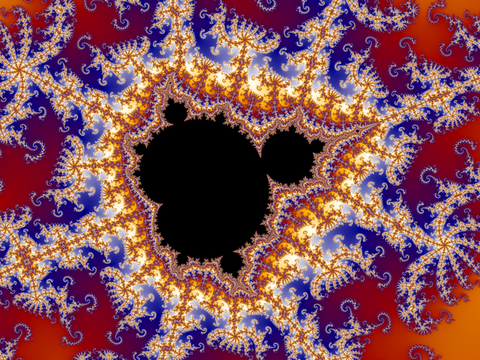
\includegraphics[width=0.5\textwidth]{mandelbrot}
  \par
\end{frame}


\section{Platonic solids}

\newcommand{\solid}[5]{\begin{column}{0.31\textwidth}\centering\hil{#2}\par#5 v, #4 e, #3 f\\\medskip\includegraphics[height=0.7\textwidth]{#1}\end{column}}
\newcommand{\solidd}[3]{\begin{column}{0.4\textwidth}\centering\hil{#2}\par#3\\\medskip\includegraphics[height=1.9cm]{#1}\end{column}}
\newcommand{\solidde}[3]{\begin{column}{0.33\textwidth}\centering\hil{#2}\par{\scriptsize#3\\}\medskip\includegraphics[height=1.9cm]{#1}\end{column}}
\newcommand{\solidv}[1]{\begin{column}{0.3\textwidth}\centering\hil{$\phantom{A}$}\par$\phantom{A}$\\\medskip\video{images/#1.mp4}{1.9cm}\end{column}}


\subsection{In 3d}

\begin{frame}{Platonic solids in 3d}
  \begin{columns}[c]
    \solid{tetrahedron}{Tetrahedron}{4}{6}{4}
    \solid{hexahedron}{Hexahedron}{6}{12}{8}
    \solid{octahedron}{Octahedron}{8}{12}{6}
  \end{columns}
  \bigskip
  \begin{columns}[c]
    \solid{dodecahedron}{Dodecahedron}{12}{30}{20}
    \solid{icosahedron}{Icosahedron}{20}{30}{12}
  \end{columns}
\end{frame}


\subsection{In 4d}

\begin{frame}{Platonic solids in 4d}
  \only<1>{
    \begin{columns}[c]
      \solidd{tetrahedron}{Tetrahedron}{4v, 6e, 4f}
      \solidd{005-cell}{Pentachoron}{5v, 10e, 10f, 5c}
      \solidv{005-cell}
    \end{columns}
  }

  \only<2>{
    \begin{columns}[c]
      \solidd{hexahedron}{Hexahedron}{8v, 12e, 6f}
      \solidd{008-cell}{Octachoron}{16v, 32e, 24f, 8c}
      \solidv{008-cell}
    \end{columns}
    \vspace*{2em}
    \begin{columns}[c]
      \solidd{octahedron}{Octahedron}{6v, 12e, 8f}
      \solidd{016-cell}{Hexadecachoron}{8v, 24e, 32f, 16c}
      \solidv{016-cell}
    \end{columns}
  }

  \only<3>{
    \begin{columns}[c]
      \solidd{dodecahedron}{Dodecahedron}{20v, 30e, 12f}
      \solidd{120-cell}{Hecatonicosachoron}{600v, 1200e, 720f, 120c}
      \solidv{120-cell}
    \end{columns}
    \vspace*{2em}
    \begin{columns}[c]
      \solidd{icosahedron}{Icosahedron}{12v, 30e, 20f}
      \solidd{600-cell}{Hexacosichoron}{120v, 720e, 1200f, 600c}
      \solidv{600-cell}
    \end{columns}
  }

  \only<4-5>{
    \centering
    \hil{Icositetrachoron}\par
    24v, 96e, 96f, 24c\\\medskip
    \only<4>{\includegraphics[width=0.5\textwidth]{024-cell}}
    \only<5>{\video{images/024-cell.mp4}{0.5\textwidth}}
  }
\end{frame}

\begin{frame}{Tesselation}
  \centering
  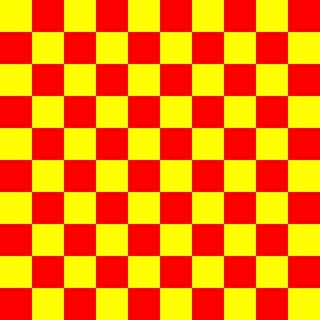
\includegraphics[height=0.6\textheight]{tesselation-squares}
  \qquad
  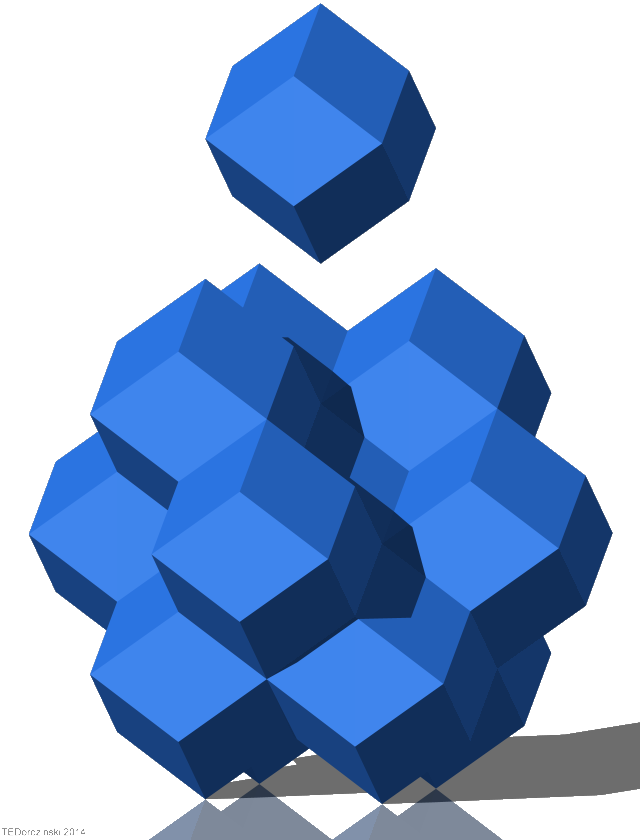
\includegraphics[height=0.6\textheight]{hyperdiamond-3d}
  \bigskip

  \hil{The 24-cell tesselates four-dimensional space.}
\end{frame}

\begin{frame}{Overview}
  \begin{columns}[c]
    \solidde{005-cell}{Pentachoron}{5v, 10e, 10f, 5c}
    \solidde{008-cell}{Octachoron}{16v, 32e, 24f, 8c}
    \solidde{016-cell}{Hexadecachoron}{8v, 24e, 32f, 16c}
  \end{columns}
  \bigskip
  \bigskip
  \begin{columns}[c]
    \solidde{120-cell}{Hecatonicosachoron}{600v, 1200e, 720f, 120c}
    \solidde{600-cell}{Hexacosichoron}{120v, 720e, 1200f, 600c}
    \solidde{024-cell}{Icositetrachoron}{24v, 96e, 96f, 24c}
  \end{columns}
\end{frame}


\subsection{In arbitrary dimensions}

\begin{frame}{In arbitrary dimensions}
  \centering
  \begin{tabular}{ll}
    \toprule
    dimension & number of Platonic solids \\ \midrule
    $n = 1$ & 1 (just the line segment) \\
    $n = 2$ & $\infty$ (triangle, square, \ldots; any regular polygon) \\
    $n = 3$ & 5 \\
    $n = 4$ & 6 \\
    $n = 5$ & 3 (just the simplex, the hypercube and its dual) \\
    $n = 6$ & 3 (just the simplex, the hypercube and its dual) \\
    $n = 7$ & 3 (just the simplex, the hypercube and its dual) \\
    \emph{and so on} \\
    \bottomrule
  \end{tabular}
  \par
\end{frame}

\note{
  \begin{itemize}
    \item The only platonic solid which can be used to tesselate
    three-dimensional space is the cube.
    \item In four dimensions, both the tesseract and the 24-cell work.
    \item This has a deeper reason: In any dimension~$n$, the $n$-dimensional
    analogue of the rhombic dodecahedron can be used to tesselate
    $n$-dimensional space. In dimension $n = 3$ the rhombic dodecahedron is not
    a Platonic solid; in dimension $n = 4$ it is (and is also called the
    ``24-cell'').
  \end{itemize}
}


\subsection[Glueing]{Glueing four-dimensional shapes}

\begin{frame}{Glueing four-dimensional shapes}
  \centering
  \begin{columns}
    \begin{column}{0.3\textwidth}
      \centering
      \hil{Cube} \\
      \smallskip
      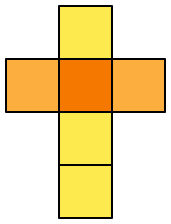
\includegraphics[height=0.35\textheight]{cube-net}
    \end{column}
    \begin{column}{0.3\textwidth}
      \centering
      \hil{Tesseract} \\
      \smallskip
      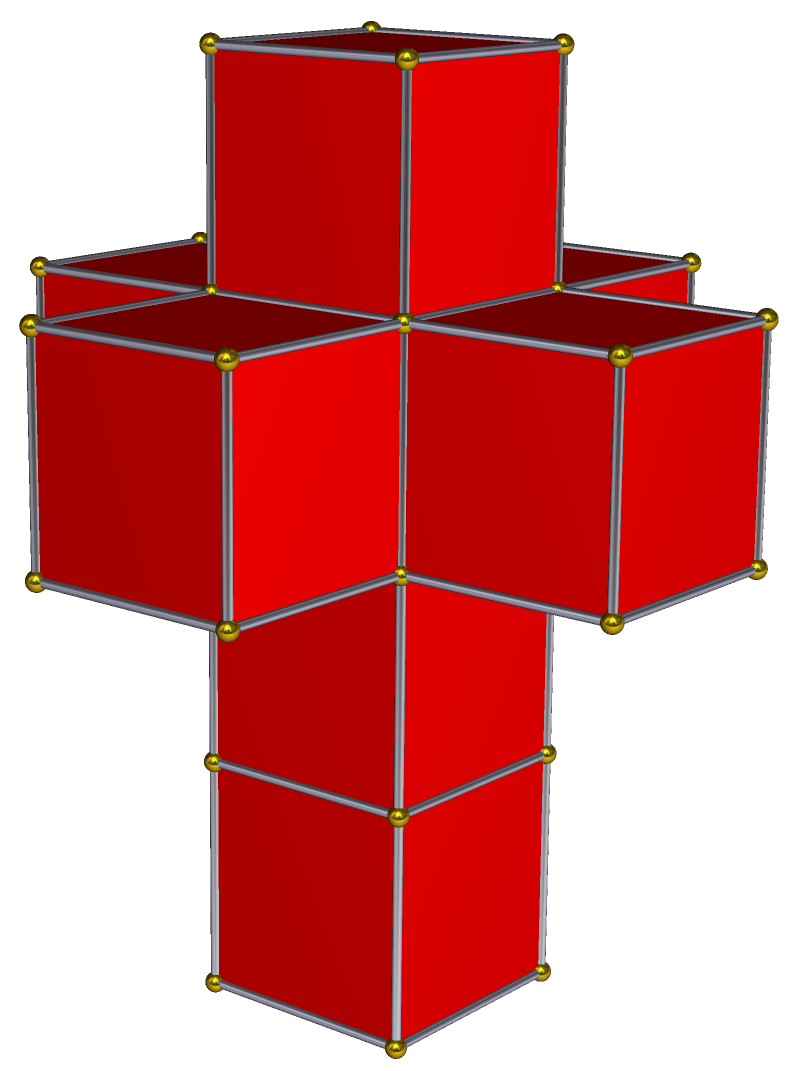
\includegraphics[height=0.35\textheight]{008-cell-net}
    \end{column}
  \end{columns}
  \bigskip
  \bigskip

  \begin{columns}
    \begin{column}{0.3\textwidth}
      \centering
      \hil{16-cell} \\
      \smallskip
      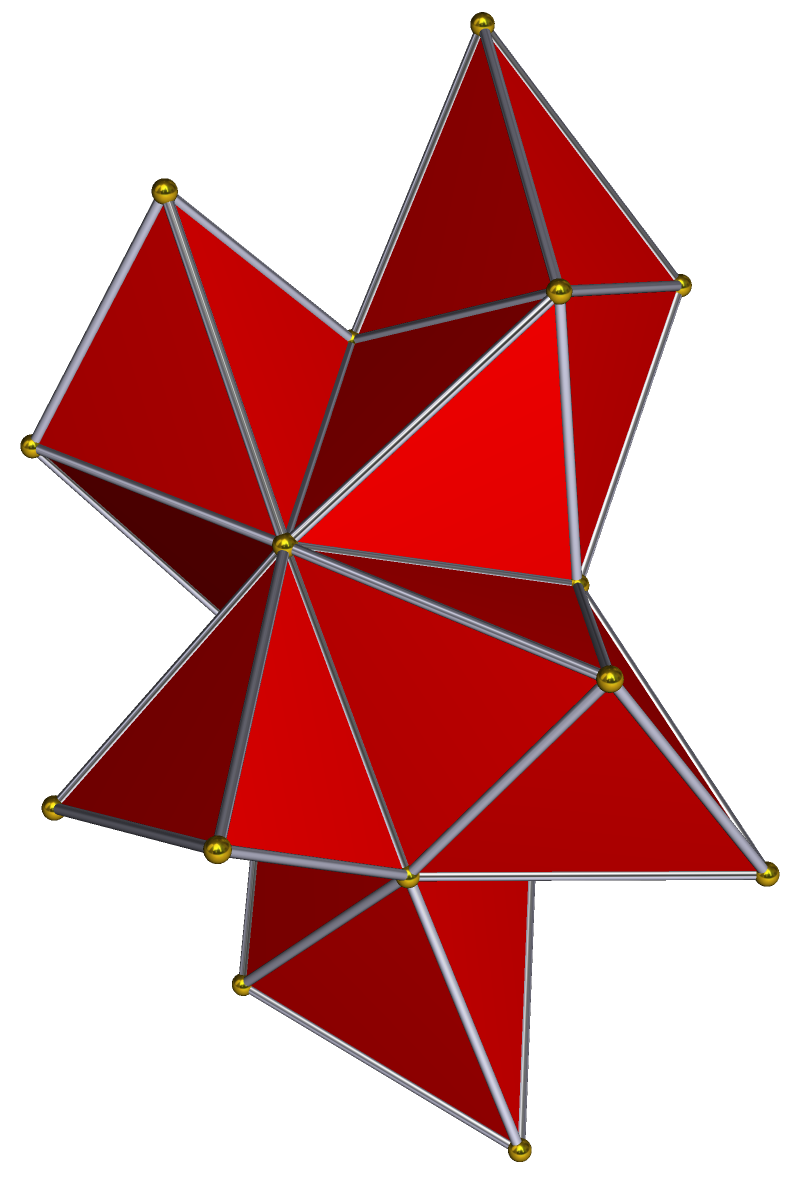
\includegraphics[height=0.3\textheight]{016-cell-net}
    \end{column}
    \begin{column}{0.3\textwidth}
      \centering
      \hil{24-cell} \\
      \smallskip
      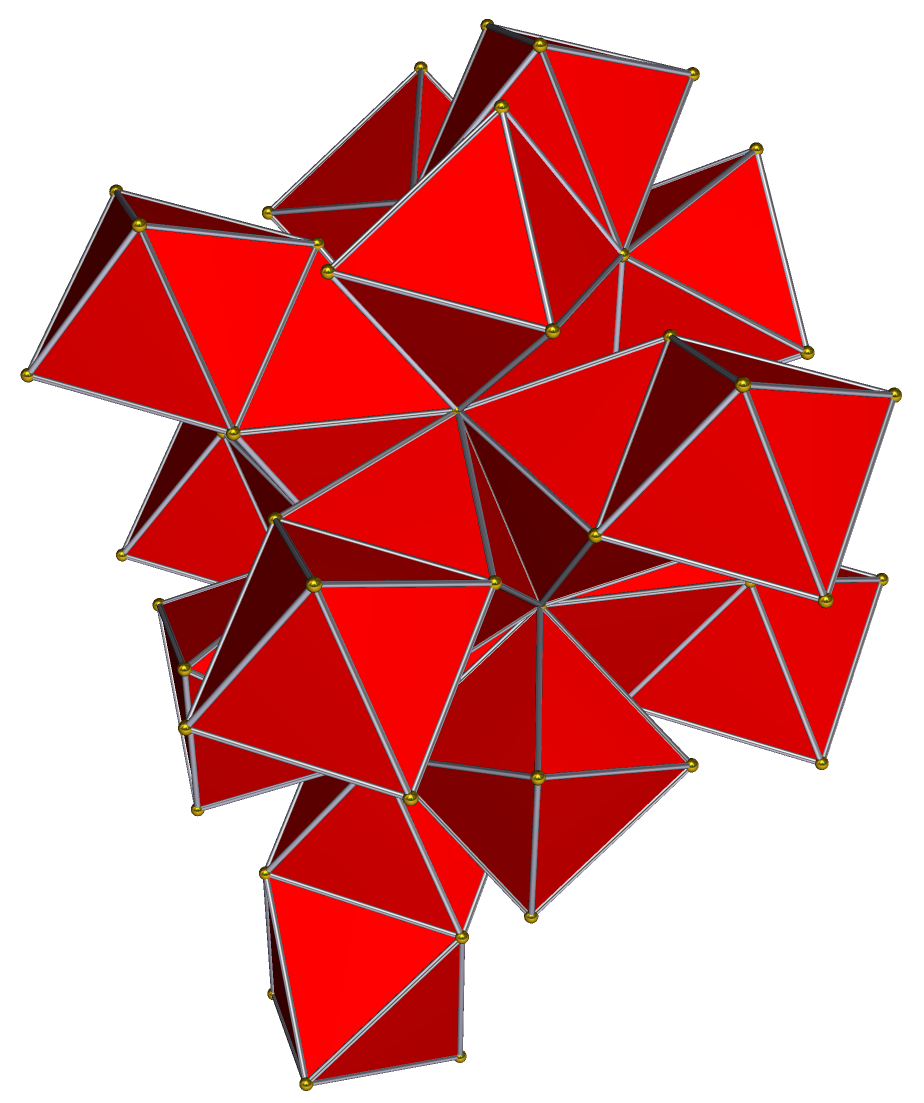
\includegraphics[height=0.3\textheight]{024-cell-net}
    \end{column}
  \end{columns}
\end{frame}

\begin{frame}[plain]
  \centering
  \medskip
  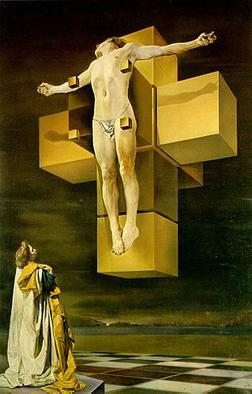
\includegraphics[height=0.95\textheight]{salvador-dali} \\
  \scriptsize
  Salvador Dalí: \hil{Corpus Hypercubus} (1954)
\end{frame}

\begin{frame}{A four-dimensional labyrinth}
  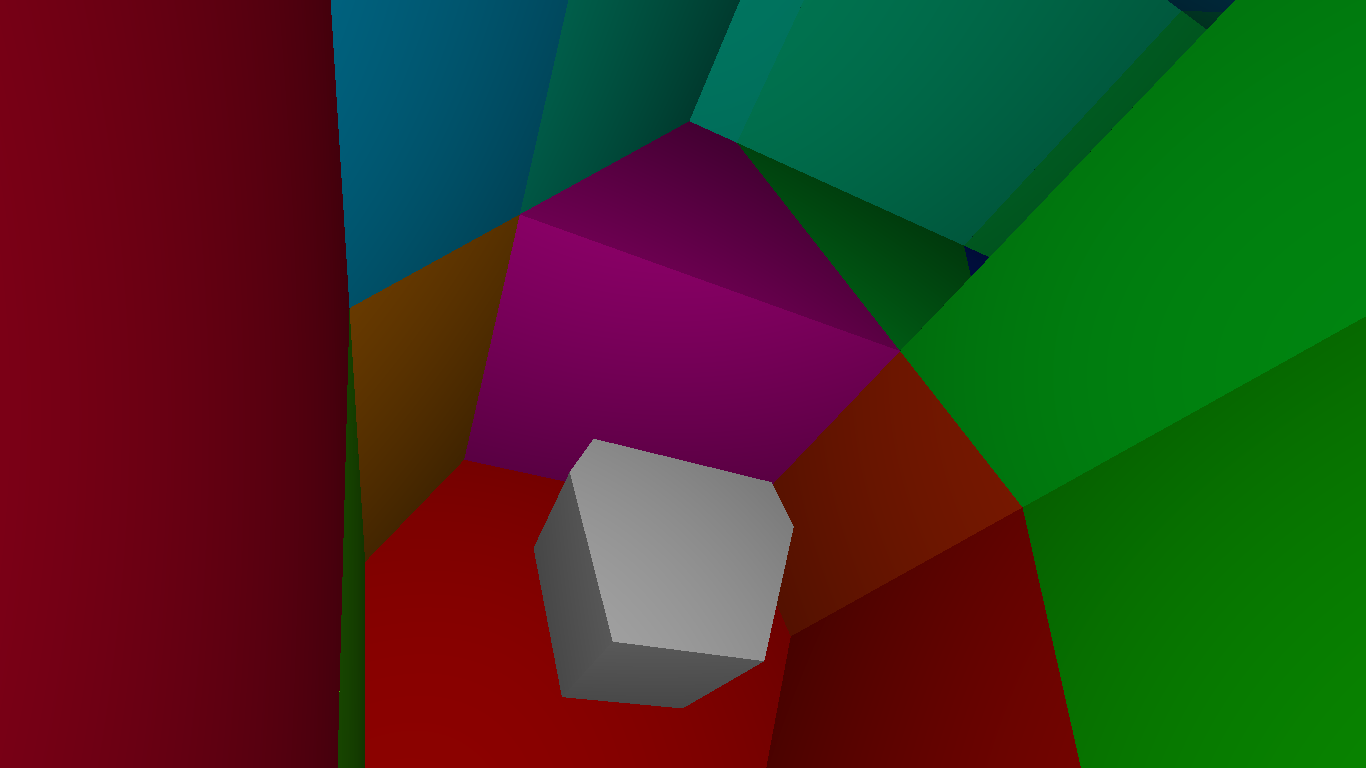
\includegraphics[width=\textwidth]{4d-labyrinth}
\end{frame}


\subsection{Outlook}

\begin{frame}{The fourth dimension \ldots}
  \begin{enumerate}
    \item is intriguingly beautiful,

    \item helps at understanding the third dimension,

    \begin{center}
      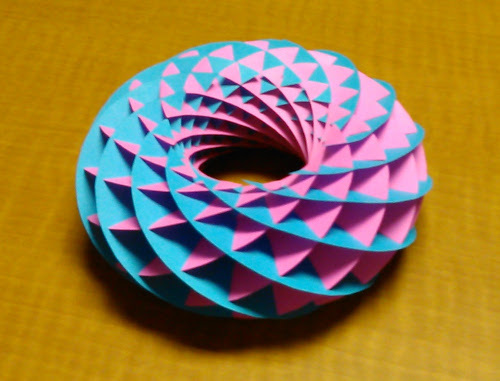
\includegraphics[height=0.3\textheight]{torus-circles}
      \qquad\qquad
      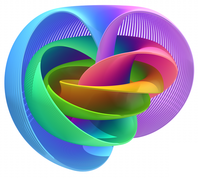
\includegraphics[height=0.3\textheight]{hopf-fibration}
    \end{center}

    \item is indispensible for modern physics,

    \item is the only dimension which is still largely not understood.

    \begin{center}
      \begin{tabular}{l|rrrrrrrrrr}
        Dimension & 1 & 2 & 3 & 4 & 5 & 6 & 7 & 8 & 9 & \ldots \\
        Number of spheres & 1 & 1 & 1 & \hil{??} & 1 & 1 & 28 & 2 & 8 & \ldots
      \end{tabular}
    \end{center}
  \end{enumerate}
\end{frame}

\begin{frame}[plain,c]
  \centering
  \begin{columns}
    \begin{column}{0.4\textwidth}
      \centering
      \hil{Catharina Stroppel} \\
      $\phantom{\text{g}}$knot theorist$\phantom{\text{g}}$ \\
      \smallskip
      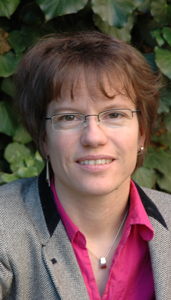
\includegraphics[height=0.5\textheight]{catharina-stroppel}
    \end{column}
    \begin{column}{0.6\textwidth}
      \centering
      \hil{Julia Grigsby} \\
      low-dimensional topologist \\
      \smallskip
      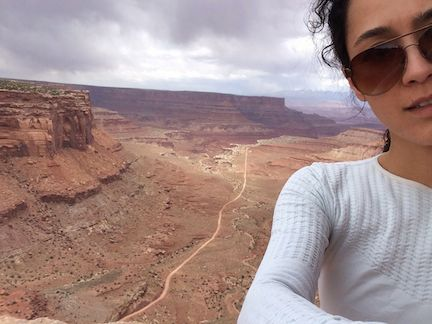
\includegraphics[height=0.5\textheight]{julia-grigsby}
    \end{column}
  \end{columns}
\end{frame}

\newcommand{\hero}[2]{\hil{#2}\\\smallskip\includegraphics[height=4cm]{#1}}
\newcommand{\specialhero}[2]{\hil{#2}\\\smallskip\includegraphics[height=5cm]{#1}}
\newcommand{\two}[2]{
  \begin{columns}
    \begin{column}{0.4\textwidth}
      \centering
      #1
    \end{column}
    \begin{column}{0.4\textwidth}
      \centering
      #2
    \end{column}
  \end{columns}
}

\begin{frame}{Applause for our heros!}
  \centering
  \only<1>{\hero{005-cell}{Pentachoron}}
  \only<2>{\two{\hero{008-cell}{Tesserakt}}{\hero{016-cell}{Hexadecachoron}}}
  \only<3>{\two{\hero{120-cell}{Hecatonicosachoron}}{\hero{600-cell}{Hexacosichoron}}}
  \only<4>{\specialhero{024-cell}{Icositetrachoron}}
  \bigskip

  \only<4>{
    Slides and programs: \\
    \hil{http://4d.speicherleck.de/} \\
    (sorry for http)
  }
\end{frame}

\appendix

\section{Image sources}

\begin{frame}{Image sources}
  \tiny

  \only<1>{Rendered images of four-dimensional bodies created by Robert Webb with his
  Stella software: \\
  \url{https://en.wikipedia.org/wiki/File:Ortho_solid_011-uniform_polychoron_53p-t0.png} \\
  \url{https://en.wikipedia.org/wiki/File:Schlegel_wireframe_5-cell.png} \\
  \url{https://en.wikipedia.org/wiki/File:Schlegel_wireframe_8-cell.png} \\
  \url{https://en.wikipedia.org/wiki/File:Schlegel_wireframe_16-cell.png} \\
  \url{https://en.wikipedia.org/wiki/File:Schlegel_wireframe_24-cell.png} \\
  \url{https://en.wikipedia.org/wiki/File:Schlegel_wireframe_120-cell.png} \\
  \url{https://en.wikipedia.org/wiki/File:Schlegel_wireframe_600-cell_vertex-centered.png}}

  \only<2>{Miscellaneous pictures: \\
  \url{http://4.bp.blogspot.com/_TbkIC-eqFNM/S-dK9dd1cUI/AAAAAAAAFjA/d8qdTHhKy1U/s320/tesseract+unfolded.png} \\
  \url{http://gwydir.demon.co.uk/jo/tess/optical6.gif}
  \url{https://commons.wikimedia.org/wiki/File:Blue_Trefoil_Knot.png} \\
  \url{https://en.wikipedia.org/wiki/File:Dodecahedron.svg} \\
  \url{https://en.wikipedia.org/wiki/File:Hexahedron.svg} \\
  \url{https://en.wikipedia.org/wiki/File:Icosahedron.svg} \\
  \url{https://en.wikipedia.org/wiki/File:Octahedron.svg} \\
  \url{https://en.wikipedia.org/wiki/File:Tetrahedron.svg} \\
  \url{https://mathlesstraveled.files.wordpress.com/2017/01/villarceau-torus-small.jpg} \\
  \url{https://upload.wikimedia.org/wikipedia/commons/1/1e/600-cell.gif} \\
  \url{https://upload.wikimedia.org/wikipedia/commons/2/24/HC_R1.png} \\
  \url{https://upload.wikimedia.org/wikipedia/commons/7/72/Rhombic_dodecahedra_b.png} \\
  \url{https://upload.wikimedia.org/wikipedia/commons/a/a0/16-cell.gif} \\
  \url{https://upload.wikimedia.org/wikipedia/commons/c/cf/Hexahedron_flat_color.svg} \\
  \url{https://upload.wikimedia.org/wikipedia/commons/d/d6/8-cell-orig.gif} \\
  \url{https://upload.wikimedia.org/wikipedia/commons/d/d8/5-cell.gif} \\
  \url{https://upload.wikimedia.org/wikipedia/commons/f/f4/24-cell.gif} \\
  \url{https://upload.wikimedia.org/wikipedia/commons/f/f9/120-cell.gif} \\
  \url{https://upload.wikimedia.org/wikipedia/commons/thumb/b/b9/Hopf_Fibration.png/250px-Hopf_Fibration.png} \\
  \url{https://upload.wikimedia.org/wikipedia/en/0/09/Dali_Crucifixion_hypercube.jpg} \\
  \url{https://www2.bc.edu/julia-grigsby/Eli_Moab_6in.JPG} \\
  \url{http://www.gnuplotting.org/figs/klein_bottle.png} \\
  \url{http://www.math.uni-bonn.de/ag/stroppel/Picture_cs2.jpg}}
\end{frame}
\addtocounter{framenumber}{-1}

\end{document}


Ecken:     2 4  8 16
Kanten:    1 4 12 32    32 = (16 * 4) / 2    12 = (8 * 3) / 2
Flächen:   0 1  6 24    (3über2)*8/4 = 6     (4über2)*16/4 = 24 = 2^2 * (4über2)
Volumina:  0 0  1  8
4-Vol.:    0 0  0  1

* Raumzeit in 2+1 Dimensionen ist schlecht wegen: Feldgleichung hat zu wenig
  Unbekannte. Masse müsste immer Null sein. (?)
* Kommutativität von gewissen Rotationen; Verknüpfungen von Rotationen ist nicht
  unbedingt Rotation (einer Ebene)! (?)
* (Rotationen nicht um Achsen, sondern "um Ebenen"; besser: Man rotiert immer "in
  einer Ebene".)
* Quaternionen?
* Ist jedes Element der SO(4) eine Rotation einer Ebene? Nein. (-Id)
* Ist jedes Element der SO(4) Verknüpfung zweier Spiegelungen an Hyperebenen? Nein.

Man könnte den Vortrag auch mit dem bekannten Witz (Mathematikerin, Physikerin,
Konferenz, Schwierigkeit, ganz einfach: dann n gegen 11) beginnen. Und dann
gleich dazu sagen, dass es bei uns um räumliche Dimensionen geht.
